\chapter{Background}
\section{Category Theory}
\subsection{Categories}

A category formally is a collection of objects and morphisms that follow a composition law \cite{context}. \todo{Expand on this. Should I give an actual definition of an abstract category? I probably should}

While this definition is very abstract, it is useful in describing a lot of things \todo{find a better word} in mathematics.
Some of the most useful categories for application are \emph{concrete} categories, which practically are categories whose objects spaces with some form of structure and morphisms are structure preserving mappings between them.


\missingfigure{Make a diagram to represent a few objects/morphisms in $\Set$.}
\missingfigure{Make a diagram to represent a few objects/morphisms in $\FinVect$. Make it look congruent to $\Set$.}

An example is shown in $\Set$ and $\FinVect$.
The category $\Set$ has sets as its objects, and its morphisms are functions.
The category $\FinVect$ has as its objects finite dimensional vector spaces over the real numbers as their bed of scalars, and its morphisms are linear transformations\footnote{These transformations can be represented by a matrix, but only if a basis is provided for both domain and codomain. We should not automatically assume a vector space has a canonical basis that's best for the job!}.
Note that $\FinVect$ is just a subcategory\footnote{I won't define it, but I hope it's not hard to imagine what a subcategory is. Closure under composition is the main requirement.} of $\Set$. This is talked about in more detail in books.\todo{Specify}

This view is different from a set theoretic approach to fields in mathematics.
For instance, the set theoretic approach to linear algebra would define a vector space as a set with a certain algebraic structure, and a linear transformation as a function preserving that structure in a certain way.
A categorical approach would instead define the category of vector spaces as a collection of objects (the vector spaces) and of morphisms\footnote{and of functors. more on that later}, and would specify how morphisms behave in composition.
This approach is described as "context rich and content poor"\todo{cite youtube video}
\todo[inline]{Finish this paragraph. Element poor, but we can get around that, and the language is unified to describe similar phenomena in different fields, blah blah blah}

\todo[inline]{Talk about functional programming}
\todo[inline]{Talk about how Markov categories are cats with markov kernels}

\subsection{Functors}
\subsubsection{Example Functors}
\subsection{Monoidal Functors}
\subsection{Natural Transformations}
\subsection{Monads}
\subsection{Kleisli Categories}

\section{Markov Categories}

Markov categories are categories in which the morphisms behave like stochastic kernels.
There are in fact Markov categories that have too restrictive of a structure to represent the probability we're interested in, but we can build a Markov category out of the kernels that we model problems with for computation.
When we formulate problems in terms of Markov categories, we can then revert to the language of category theory and abstract away the details of which computations the morphisms in a particular Markov category represent.

More specifically, a good way to think about a Markov category is that the objects represent classes of distributions\footnote{While most of the time objects are enumerated by the underlying statespace (or dimension for that matter), it's helpful to think of them as the collections of distributions themselves}, and the morphisms are mappings between them.

For example, the spaces and mappings discussed in Section \ref{the kalman filter kernels section} form the Markov category $\gausscat$.
Each object is $\gaussian X$, the collection of Gaussian distributions on the vector space $X$.
The morphisms are the kernels specified in Equations \ref{gaussian kernels}.

\subsection{Definition}

A Markov category is a symmetric monoidal category with comonoidal objects.

\subsection{Example: Set}
\subsection{Kleisli Categories}

\section{String Diagrams}

String diagrams are very similar to the signal flow diagrams or block diagrams found in control systems.
Others (\cite{baez2015control}, \cite{fong2016thesis}, \cite{fong2016dynamicalsystems}) have drawn the connections between string diagrams and various diagrams in systems engineering including block diagrams for dynamical systems.

There are often two interpretations in block diagrams:
In what I will call the temporal interpretation, the state of a diagram can be seen as changing over time, where the states are carried by the wires from block to block. The blocks represent state transformations, which are applied continuously to their inputs to generate changing outputs.
There may be blocks which carry their own internal state, such as integrators, that keep track of quantities over time to affect their output\todo{This sentence sucks.}

In what I'll call the signal flow interpretation, a time-varying signal is seen as a single entity, and the blocks represent signals in transformation space. This interpretation allows for a more functional analysis type approach to control design.

String diagrams look quite similar to block diagrams, but their interpretation is very different.
Blocks are still seen as transformations, but they then become the primary point of interest instead of the "signals" themselves.
The wires do not represent signals, but rather state spaces.
Whenever a wire splits, or disappears, or loops around, that becomes interpreted as a special transformation itself.
With this interpretation, a string diagram simply becomes a tool to draw out complicated compositions of transformations, or morphisms in a symmetric monoidal category.

\subsection{Explanation of String Diagrams}

\subsection{Translating String Diagrams into Kernel Compositions}
String diagrams allow us to write complicated equations with a single picture that can then be systematically translated back into equations for computation.
These pictures are often much clearer to interpret, and easier to memorize as they can be puzzle pieced together.
Interpreting them is straightforward: Take the example problem of finding the conditional of a kernel with respect to part of its output.
This problem statement carries with it the nuance of the complexity in finding conditionals, unlike the simple measure theoretic definition.

Given $f:A\rightarrow X\otimes Y$, find $f_X : X\otimes A \rightarrow Y$ such that the equation in Figure \ref{fig:conditional} holds.

\begin{figure}[htb]
	\centering
	\tikzfig{conditional}
	\caption{The string diagram equation for the definition of conditioning.}
	\label{tikz:conditional}
\end{figure}

\begin{figure}[htb]
	\centering
	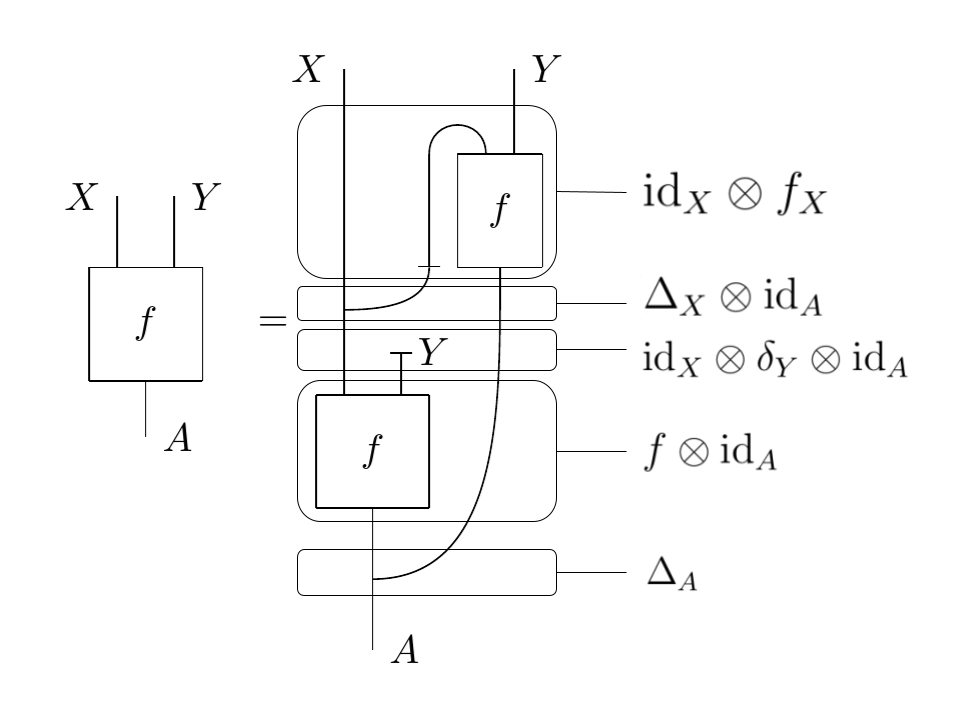
\includegraphics[width=0.8\textwidth]{conditional-compositions}
	\caption{The conditional equation is read like so. This corresponds to Equation \ref{eq:conditional-compositions}.}
	\label{fig:conditional-compositions}
\end{figure}

\begin{figure}[htb]
	\centering
	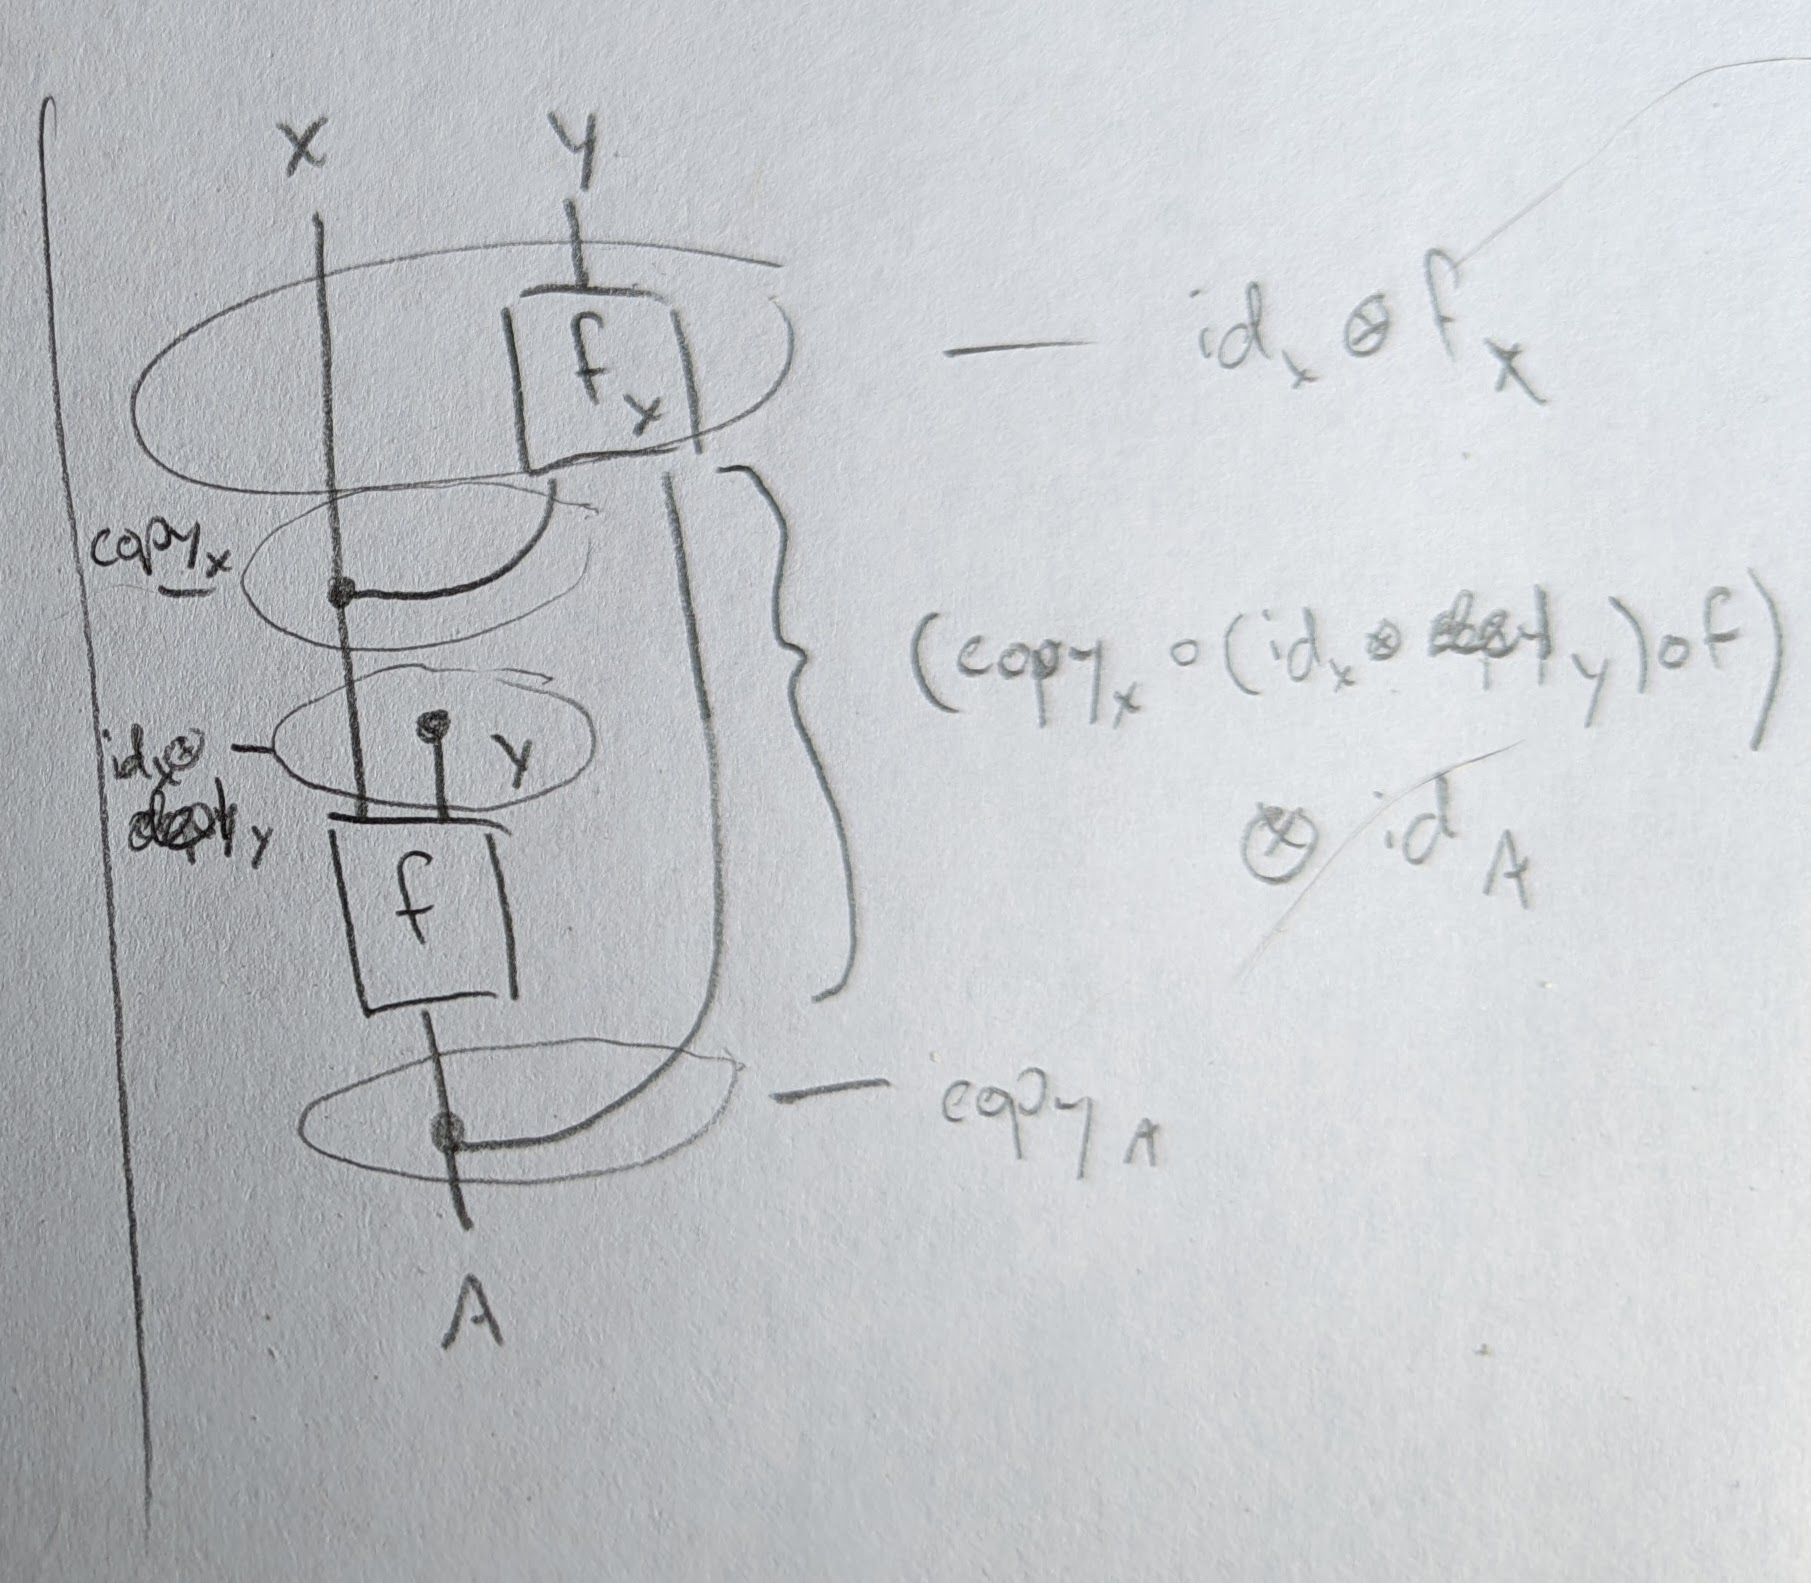
\includegraphics[width=0.5\textwidth]{conditional-parallel-compositions}
	\caption{The conditional equation can also be read this way. This corresponds to Equation \ref{eq:conditional-parallel-compositions}.}
	\label{fig:conditional-parallel-compositions}
\end{figure}

\begin{equation}
\label{eq:conditional-compositions}
f = (\id_X \otimes f_X) \circ (\comul_X \otimes \id_A)
\circ (\id_X \otimes \counit_Y \otimes \id_A) \circ (f \otimes \id_A) \circ \comul_A
\end{equation}

\begin{equation}
\label{eq:conditional-parallel-compositions}
f = (\id_x \otimes f_x) \circ \left[\left(\comul_x \circ (\id_x\otimes \counit_Y) \circ f\right) \otimes \id_A\right] \circ \comul_A
\end{equation}

** Explain notation. Every operator you are using in these equations should be explained and formally introduced. **

\section{Bar Notation}
\subsection{Explanation of Bar Notation}
\subsection{Translating Bar Notation into String Diagrams}

\chapter{Common Representations of Information Recast into the Language of Markov Categories}
\section{Discrete Probability}
\section{Gaussian Probability}
\section{Gaussian Mixtures: A Composition of Discrete and Gaussian Probability}

The framework in this section was developed with much help from Tobias Fritz in the Category theory Zulip channel \cite{zulip}

We now develop Gaussian mixtures in purely abstract terms.
First let's discuss Gaussian mixtures concretely.

A basic explanation of Gaussian mixtures is that a Gaussian mixture distribution is a convex combination of Gaussian distributions.
More formally, if we have $p_i: I\rightarrow X$, then a Gaussian mixture distribution can be defined as
\begin{equation}
    p = \sum_i w_i | p_i \rangle
\end{equation}
where every $w_i \geq 0$, and $\sum_i w_i = 1$.
Here we use the ket notation as in \cite{cho-jacobs}.
This can be interpreted as a point-wise summation on the PDFs of the Gaussians, or we can keep it as a formal sum ie.\ a sequence of pairs.

Notice that the collection of these convex combinations is precisely the finite distribution monad $\distributionmonad$ applied not to the space $X$, but seemingly to the collection of Gaussians $\gaussian X$.

\subsection{Distributive Laws}

A first approach would to be try distributive laws.
In essence, these allow you to compose monads.
This unfortunately will not work for Gaussian mixtures for several reasons, but this can still yield us new Markov categories by combining old ones.

Given two monads $(S,\mu^S, \eta^S)$ and $(T, \mu^T,\eta^T)$, a distributive law of $S$ over $T$ is a natural transformation
\begin{equation}
    l:TS\rightarrow ST
\end{equation}
satisfying certain conditions. \todo{Should I write these conditions? Probably if I want to prove the following.}

An important feature here is that we can compose the monads, at least in one direction as $ST$, to form a new monad.
In partcular, the join and unit NTs become
\begin{align}
    \mu^{ST} &: STST \xrightarrow{SlT} SSTT \xrightarrow{\mu^S \mu^T} ST\\
    \eta^{ST} &: 1\xrightarrow{\eta^S\eta^T}ST
\end{align}

Remember that Markov categories arise from symmetric monoidal affine monads on other Markov categories.
Thus, if $T,\ S\in C$ are symmetric monoidal affine monads, with laxators $\laxator^T$ and $\laxator^S$ respectively, then $ST$ will\todo{prove this} become symmetric monoidal affine with
\begin{equation}
    \laxator^{ST}_{X,Y} : STX \otimes STY \xrightarrow{\laxator^S_{TX,TY}}
    S(TX\otimes TY) \xrightarrow{S\laxator^T_{X,Y}} ST(X\otimes Y)
\end{equation}

Thus, we can now compose two probability monads to make a third.
Unfortunately, however, this will not help us with Gaussian mixtures.
For one, $\gaussian$ is not an endofunctor, and $\gausscat$ is not a Kleisli category.
We simply abuse the notation for convenience.
And even if we were to try to treat $\gaussian$ as an endofunctor, the composition wouldn't make sense.
The distributive law $l$ requires the functor compositions to go both ways. 
It would make sense to construct $\distributionmonad\gaussian X$ as a convex combination of Gaussian distributions on $X$, but not so much for $\gaussian \distributionmonad X$, a Gaussian distribution of convex combinations of $X$'s.

Still, we should push this further. Let's try to come up with conditioning on $ST$.
\todo[inline]{Dr. Bakolas this is where I need help}

\subsection{Markov functor}

What if we have a Markov functor to another Markov category, and then apply a monoidal monad to its image?
This should work, but it still won't give us what we want I don't think.

\subsection{Monads Applied to Hom Sets}

One way that will work with Gaussian mixtures is to use a hom set construction.

If we consider a Markov category $C$, then the space of distributions on $X\in C$ is equivalent to the hom set $C(1,X)$.

\chapter{Programming with Markov Categories}
\section{Making Datatypes}
\subsection{Gaussian}
\subsection{Unscented}
\subsection{Gaussian Mixtures}


\section{Synthetic Algorithms Used in Estimation and Control}
\subsection{Filtering}
\subsection{Batch Estimation}
\subsection{History Space}
